\section{Quick Start}
\label{sec:quick_start}

% Esta seccao deve ter um pequeno tutorial a demonstrar como fazer uma
% transformacao muito simples.

% Colocar transformacao de GenealogyTree pra algum target bom.

In this section you will create the two transformations
described in page \pageref{subsubsec:metaphor} using \emph{DSLTrans} graphical
syntax.

\subsection{Metamodels}

First step is to build the required metamodels: \emph{GenealogyTree} and
\emph{Couples}. Both were built using \emph{Ecore Diagram Editor} and are shown
in figures \ref{fig:genealogy_tree_mm} and \ref{fig:couples_mm}. 

\begin{figure}[h]
\begin{center}
  \subfloat[GenealogyTree.]{\label{fig:genealogy_tree_mm}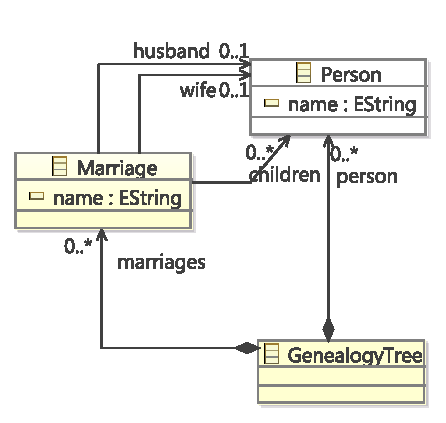
\includegraphics[width=0.45\textwidth]{imgs/GenealogyTree.pdf}}
  \subfloat[Couples.]{\label{fig:couples_mm}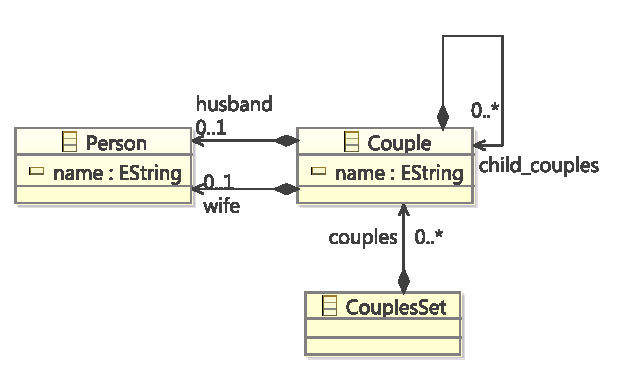
\includegraphics[width=0.45\textwidth]{imgs/Couples.pdf}}
  \caption{Metamodels.}
  \label{fig:genTree_couples_metamodels}
\end{center}
\end{figure}

Notice that in the \emph{Couples} metamodel the notion of parenting
relationship between \emph{Couples} is kept. For a given couple to be
directly connected to other couple it means that the first one gave birth to one
of the elements of the second couple.

\clearpage

\subsection{Example Model}
\label{subsec:creating_example_model}

To test the transformation you will need an example model. Open the
\emph{GenealogyTree.ecore} file and click on \emph{Create Dynamic
Instance\ldots}. Name the new file as \emph{GenealogyTree.xmi} (see figure
\ref{fig:create_dinamic_instance} ). It is important that you name it like that
to avoid confusion later in this tutorial.


\begin{figure}[h]
\begin{center}
  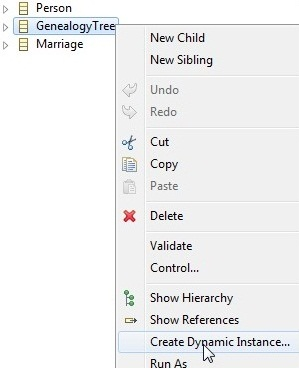
\includegraphics[scale=0.7]{imgs/create_dinamic_instance.jpg}
  \caption{Dynamic Instance Creation.}
  \label{fig:create_dinamic_instance}
\end{center}
\end{figure}

Then open the created file (\emph{GenealogyTree.xmi}) and create a model based
on figure \ref{fig:genealogy_tree_example} in page
\pageref{fig:genealogy_tree_example}. Your model should look like the one shown
in figure \ref{fig:genealogical_tree_example_model}. Don't forget to fill the
\emph{Children}, \emph{Husband} and \emph{Wife} properties (in eclipse's
properties view) for each \emph{Marriage}, where appropriate.

\begin{figure}[h]
\begin{center}
  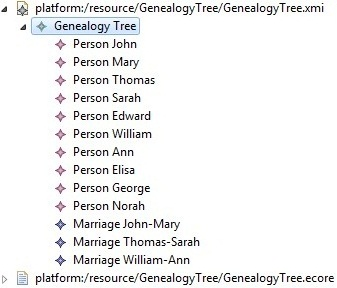
\includegraphics[scale=0.7]{imgs/genealogical_tree_example_model.jpg}
  \caption{\emph{GenealogyTree} Example Model.}
  \label{fig:genealogical_tree_example_model}
\end{center}
\end{figure}

\clearpage

\subsection{Planning the Transformation}

In page \pageref{subsubsec:metaphor} we had two ways of expressing the
transformation to generate \emph{Couples} models: a simple one and an extended,
more partitioned, version.

Informally, if we ignore the parenting relationship between couples, we can say
that a couple is a \emph{Couple} element, together with
the respective \emph{husband} and \emph{wife} \emph{Persons}. So we only have to
match the
\emph{Persons} and \emph{Marriage} elements in the \emph{GenealogyTree}
metamodel.

It is advised that before you start building the transformation, you write down
the basic rules (or steps if you prefer) that make it up. For this case study
ignore the parenting relationship between \emph{Couples} and use the following
rules:

\begin{enumerate}
  \item Every \emph{Marriage}, \emph{husband} and \emph{wife} \emph{Persons} in
  the \emph{GenealogyTree} becomes a \emph{Couple}, \emph{husband} and
  \emph{wife} \emph{Persons} in the \emph{Couples} model;
  \item Every \emph{Couple} generated has to be connected with the
  \emph{CouplesSet} (root) element.
\end{enumerate}

\clearpage

\subsection{Understanding DSLTrans Overall Semantics}

A \emph{DSLTrans} transformation is composed of multiple
\emph{layers}, each with several \emph{rules}. A \emph{rule} has a match side -
where a pattern is matched against some input model - and an apply side - where a pattern is
created in the output model. It is applied while there are elements
in the input model that satisfy the match pattern. In a \emph{layer}, all the
\emph{rules} are executed in a non-deterministic fashion while \emph{layers} are
executed sequentially following the \emph{previous source} association.

\clearpage

\subsection{Creating a Blank Transformation}

Now that you have an idea of the rules needed and how a transformation is
processed, you can start creating a blank transformation.

First open the \emph{New File Wizard} and select \emph{DSLtrans Diagram} inside
the \emph{Examples} category (see figure \ref{fig:create_dsltransformation_1}).

\begin{figure}[h]
\begin{center}
  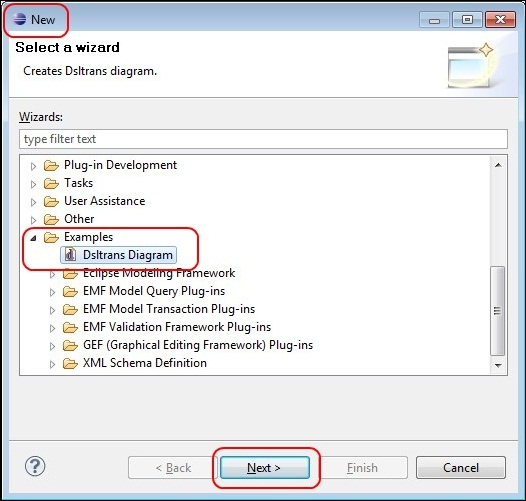
\includegraphics[scale=0.6]{imgs/create_dsltransformation_1.jpg}
  \caption{New File Wizard.}
  \label{fig:create_dsltransformation_1}
\end{center}
\end{figure}

\emph{DSLTrans} transformations are nothing but models conforming to the
\emph{DSLTrans} metamodel. According to \emph{EMF}, the abstract
definition of models is expressed in the \emph{XML Metadata
Interchange} (\emph{XMI}) \cite{xmi_omg}. Since you are using the graphical
syntax to build the transformation, the new \emph{DSLtrans Diagram} wizard will create two files:
\begin{description}
  \item[NewTransformation.dsltrans]	This file contains the transformation model
  in \emph{XMI} format. See figure \ref{fig:create_dsltransformation_3}.
  \item[NewTransformation.dsltrans\_diagram] This file contains the additional
  information needed to create and position the transformation elements in a
  diagram. See figure \ref{fig:create_dsltransformation_2}.
\end{description}

\begin{figure}[h]
\begin{center}
  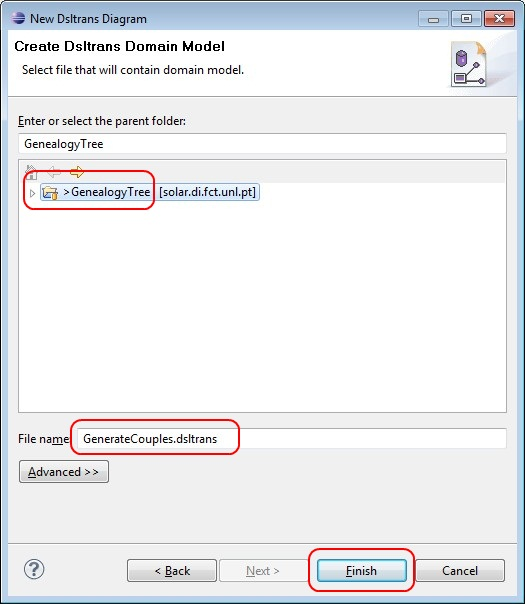
\includegraphics[scale=0.6]{imgs/create_dsltransformation_3.jpg}
  \caption{Setting model name.}
  \label{fig:create_dsltransformation_3}
\end{center}
\end{figure}

\begin{figure}[h]
\begin{center}
  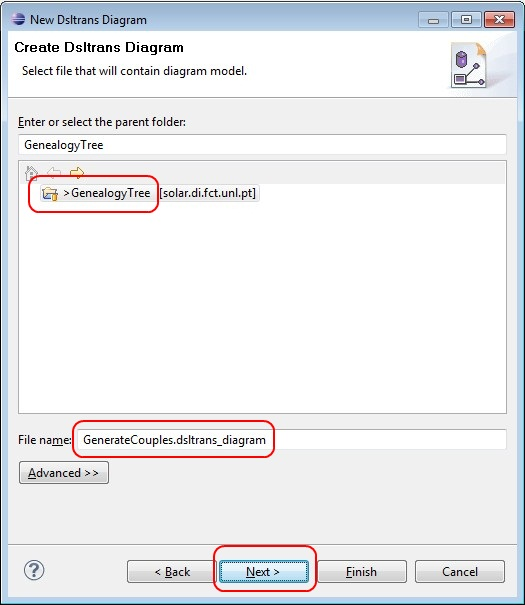
\includegraphics[scale=0.6]{imgs/create_dsltransformation_2.jpg}
  \caption{Setting diagram name.}
  \label{fig:create_dsltransformation_2}
\end{center}
\end{figure}

\clearpage

\subsection{DSLtrans Diagram Editor}

After creating and opening a new \emph{DSLTrans} file, you will see a window
like the one shown in figure \ref{fig:dsltrans_editor_window}.

While building a transformation you will frequently use:
\begin{itemize}
  \item The \emph{Properties} window to set package names and other properties
  of the transformation elements;
  \item The \emph{Palette} is used to add new elements to the transformation
  (e.g., \emph{rules}, match classes, etc\ldots) and connections among them;
  \item The \emph{Outline} view to get an idea of the overall structure of the
  transformation and navigate easily trough complex diagrams;
\end{itemize}

\begin{figure}[h]
\begin{center}
  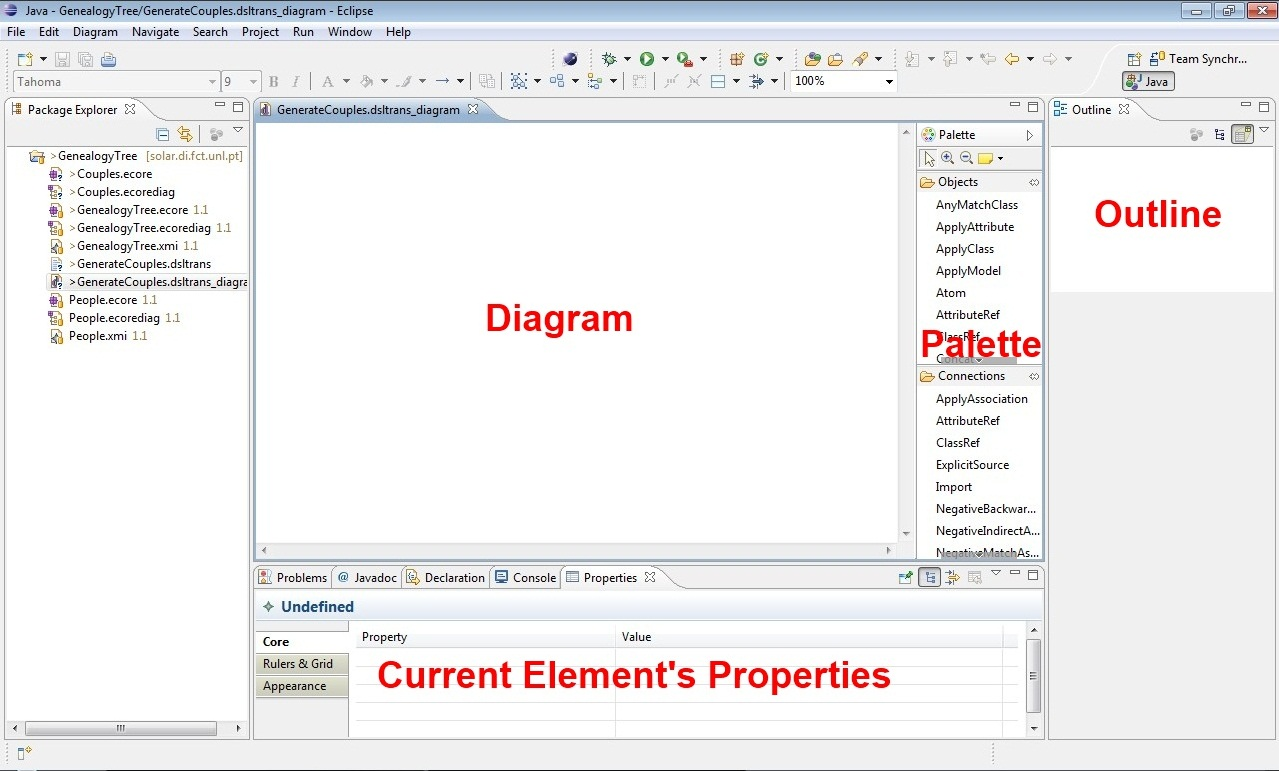
\includegraphics[width=\textwidth]{imgs/dsltrans_editor_window.jpg}
  \caption{DSLTrans Diagram Editor Window.}
  \label{fig:dsltrans_editor_window}
\end{center}
\end{figure}

\clearpage

\subsection{Defining the Transformation}

A transformation can have multiple input and output models but for this example
you only need one input and one output. To set the input for the transformation
you will add a new \emph{FilePort} by clicking it in the objects section of the
\emph{Palette} and clicking again in the diagram. After this you should see
something like figure \ref{fig:file_port_add}.


\begin{figure}[h]
\begin{center}
  \subfloat[FilePort
  Palette.]{\label{fig:click_file_port}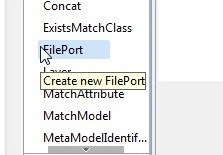
\includegraphics[width=0.3\textwidth]{imgs/click_file_port.jpg}}
  \subfloat[FilePort
  Diagram.]{\label{fig:after_click_file_port}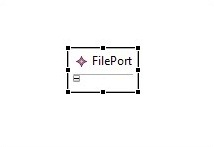
\includegraphics[width=0.3\textwidth]{imgs/after_click_file_port.jpg}}
  \caption{Adding a new element - FilePort.}
  \label{fig:file_port_add}
\end{center}
\end{figure}

Then you should set the \emph{FilePort}'s properties in the \emph{Properties}
window as in figure \ref{fig:file_port_properties}. Notice that the
\emph{Name} property can be anything. Just write something meaningful for the
sake of readability.

\begin{figure}[h]
\begin{center}
  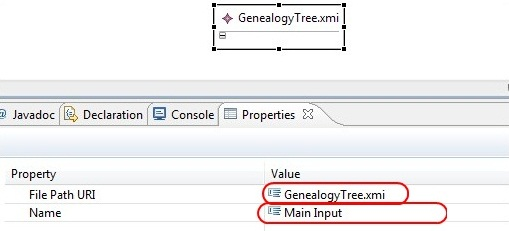
\includegraphics[scale=0.7]{imgs/file_port_properties.jpg}
  \caption{FilePort properties.}
  \label{fig:file_port_properties}
\end{center}
\end{figure}

For every input model of a \emph{DSLTrans} transformation, the metamodel it
conforms to must be stated. To do that, you add a \emph{MetaModelIdentifier}
inside the \emph{FilePort} previously created. Then set the properties as in
figure \ref{fig:meta_id_properties}.

\begin{figure}[h]
\begin{center}
  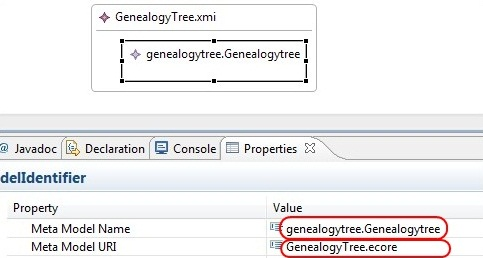
\includegraphics[scale=0.7]{imgs/meta_id_properties.jpg}
  \caption{MetaModelIdentifier properties.}
  \label{fig:meta_id_properties}
\end{center}
\end{figure}

Beware that \emph{Meta Model Name} as to be always in the format
\verb=package.Package=. The \verb=package= value is the metamodel root package
(see figure \ref{fig:package_name}). By default, this is the name of the
metamodel in lower case letters.


\begin{figure}[h]
\begin{center}
  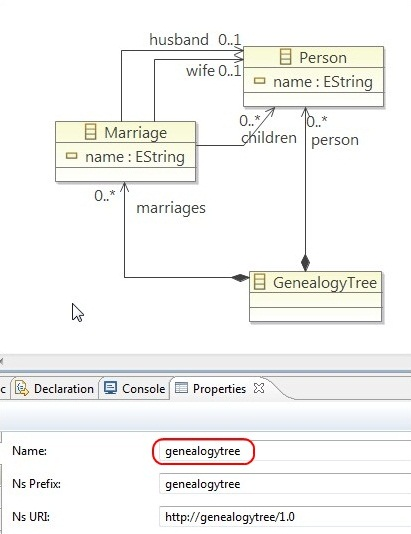
\includegraphics[scale=0.7]{imgs/package_name.jpg}
  \caption{GenealogyTree metamodel package name.}
  \label{fig:package_name}
\end{center}
\end{figure}


Now that the input is well known and identified, you can proceed to add a
first \emph{Layer} by the same procedure as described earlier to add elements to the
transformation. As for its properties it is only recommended that
you set the \emph{Name} and \emph{Description} to something meaningful.

The next step is to connect the input \emph{FilePort} to the first \emph{Layer}
using a \emph{PreviousSource} association. To add this connection you have to
first click in the \emph{PreviousSource} in the \emph{Palette}, then click in
the \emph{Layer} and drag the connection to the \emph{FilePort}. The result is
in figure \ref{fig:after_previous_source}. Don't be misled by the fact that the
arrows points downwards while you dragged it upwards. It
shows the flow of the information but its name is \emph{PreviousSource}.

\begin{figure}[h]
\begin{center}
  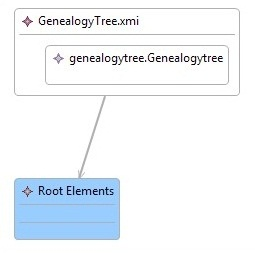
\includegraphics[scale=0.7]{imgs/after_previous_source.jpg}
  \caption{Transformation after adding the PreviousSource Association.}
  \label{fig:after_previous_source}
\end{center}
\end{figure}

Each \emph{Layer} has an output. You can set that output to a file (by setting
the \emph{Output File Path URI} property) if you want to see the outcome of the
transformation at a specific \emph{Layer}. This is great for debugging purposes.
You should set the \emph{Output File Path URI} property to \emph{Couples.xmi}.
Even if there is no external output set, the outcome of a
layer is always validated against it's metamodel. Because of it you have to
create a \emph{MetaModelIdentifier} pointing to the output metamodel for each layer.
Figure \ref{fig:metamodelid_l1} shows the properties of this
\emph{MetaModelIdentifier}.


\begin{figure}[h]
\begin{center}
  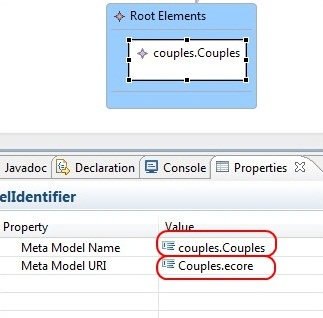
\includegraphics[scale=0.7]{imgs/metamodelid_l1.jpg}
  \caption{\emph{MetaModelIdentifier} properties.}
  \label{fig:metamodelid_l1}
\end{center}
\end{figure}


As for the rules in this \emph{layer}, we only need one: to create the root
element of the output model. It has to be like this because in the next layers
new elements will be generated and they need to be ``attached'' to the root
element as described in the \emph{Couples} metamodel. Don't worry if you can't
understand everything yet, keep going, you're almost there!

Now insert a \emph{Rule} in the recently created \emph{Layer} and set its
description to something that describes the main purpose of the \emph{Rule}
(e.g., root element). After that, insert a \emph{MatchModel} and an
\emph{ApplyModel} in the top and bottom parts of the \emph{Rule}, respectively
(see figure \ref{fig:root_elements_empty_rule}).

\begin{figure}[h]
\begin{center}
  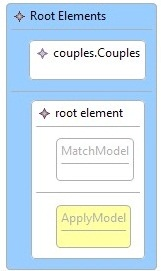
\includegraphics[scale=0.7]{imgs/root_elements_empty_rule.jpg}
  \caption{Root Elements rule with empty match and apply models.}
  \label{fig:root_elements_empty_rule}
\end{center}
\end{figure}

According to figure \ref{fig:genTree_couples_metamodels} the root element of the
\emph{GenealogyTree} metamodel is the \emph{GenealogyTree} element and the root
of the \emph{Couples} metamodel is the \emph{CouplesSet} element.

The purpose of this rule is to say that for every \emph{GenealogyTree} element
in the input model, you want to generate a \emph{CouplesSet} element in the
output model. Figure \ref{fig:rule_match_apply_class} shows the
\emph{AnyMatchClass} and the \emph{ApplyClass} elements created inside the respective containner models
created previously. As for the properties of each inserted element, set them
according to figure \ref{fig:match_apply_classes_properties}.

\begin{figure}[h]
\begin{center}
  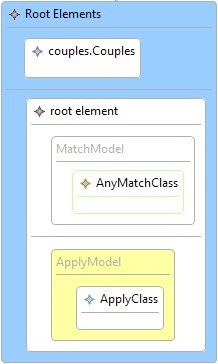
\includegraphics[scale=0.7]{imgs/rule_match_apply_class.jpg}
  \caption{AnyMatchClass and ApplyClass elements.}
  \label{fig:rule_match_apply_class}
\end{center}
\end{figure}

\begin{figure}[h]
\begin{center}
  \subfloat[GenealogyTree
  AnyMatchClass
  properties.]{\label{fig:genealogy_properties_match}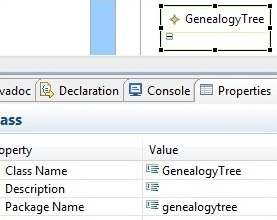
\includegraphics[width=0.35\textwidth]{imgs/genealogy_properties_match.jpg}}
  \subfloat[CouplesSet ApplyClass element
  properties.]{\label{fig:couplesset_properties_apply}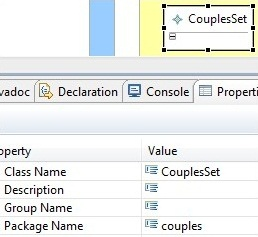
\includegraphics[width=0.35\textwidth]{imgs/couplesset_properties_apply.jpg}}
  \caption{Match and Apply Pattern properties.}
  \label{fig:match_apply_classes_properties}
\end{center}
\end{figure}

Now would be a good time to test the transformation. The transformation has one
\emph{FilePort} that points to a \emph{GenealogyTree.xmi} file where the input
model is (you created it in section \ref{subsec:creating_example_model}); and
one \emph{Layer} whose output is a file named \emph{Couples.xmi}, where the
output model will be.

To run the transformation, just right-click in
\emph{TransformationName.dsltrans}, \emph{DSLTranslator} and
\emph{Transform}, as in figure \ref{fig:transform_dsltrans}. You should see some
debugging output in the console view. If any error occurs, refer to section
\ref{sec:faq} in page \pageref{sec:faq}.

\begin{figure}[h]
\begin{center}
  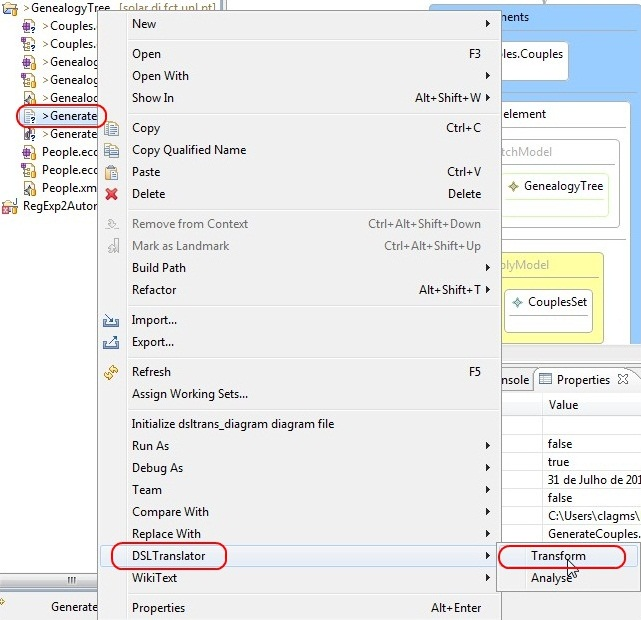
\includegraphics[scale=0.7]{imgs/transform_dsltrans.jpg}
  \caption{Executing a transformation.}
  \label{fig:transform_dsltrans}
\end{center}
\end{figure}

If everything went well you should see a new file named \emph{Couples.xmi} on
your project. Open it and you will see that the model only contains the root
element (see figure \ref{fig:couples_xmi_1}). This makes sense since the
transformation only matches \emph{GenealogyTree} elements to produce
\emph{CouplesSet} elements and there is only one \emph{GenealogyTree} element in
the input model.

\begin{figure}[h]
\begin{center}
  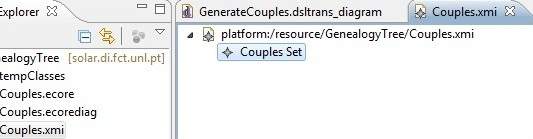
\includegraphics[scale=0.7]{imgs/couples_xmi_1.jpg}
  \caption{Couples resulting model.}
  \label{fig:couples_xmi_1}
\end{center}
\end{figure}


It's time to add a second \emph{Layer} to the transformation. Don't forget to
identify the output metamodel using the \emph{MetaModelIdentifier} as
previously. The properties of the \emph{Layer} and \emph{MetaModelIdentifier}
are the same except theres is a new \emph{Previous Source} association between
the second \emph{Layer} and the first one, as figure
\ref{fig:second_layer_empty} illustrates.

\begin{figure}[h]
\begin{center}
  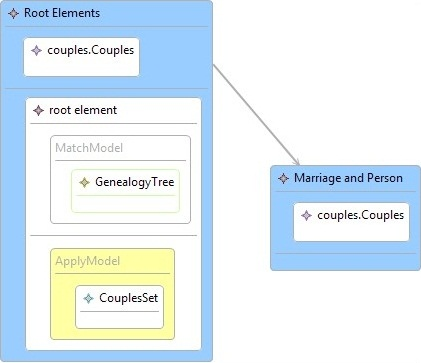
\includegraphics[scale=0.7]{imgs/second_layer_empty.jpg}
  \caption{New \emph{Layer} with \emph{Previous Source} association.}
  \label{fig:second_layer_empty}
\end{center}
\end{figure}

The second \emph{Layer} will have rules that match \emph{Marriages} in order to
generate \emph{Couples}. The skeleton of the \emph{Rule} to add is quite simple
(see figure \ref{fig:second_rule_skeleton}). Beware that you need to add
\emph{Match} and \emph{Apply} models to each side of the \emph{Rule} before
adding the \emph{AnyMatchClasses} and \emph{ApplyClasses}.

\begin{figure}[h]
\begin{center}
  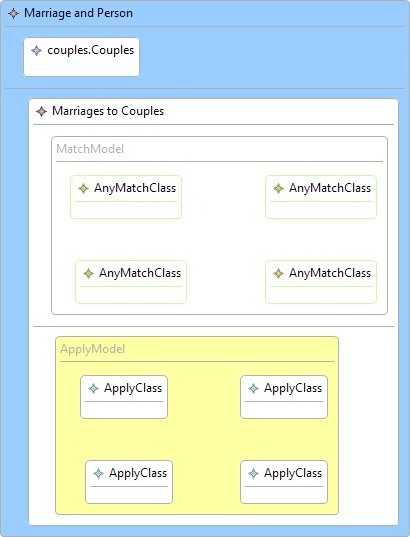
\includegraphics[scale=0.7]{imgs/second_rule_skeleton.jpg}
  \caption{Second Rule Skeleton.}
  \label{fig:second_rule_skeleton}
\end{center}
\end{figure}

On the top of the \emph{Rule} it is necessary to match a \emph{Marriage} and the
two associated \emph{Persons}, so go ahead and set the appropriate properties
for three of the four \emph{AnyMatchClasses} in the \emph{MatchModel} (see
figure \ref{fig:second_rule_skeleton_2}). Since a \emph{Couple} and two
\emph{Persons} will be generated by this \emph{Rule}, set the properties of the
\emph{ApplyCasses} according to figure \ref{fig:second_rule_skeleton_2}. It is
very important that you set the \emph{PackageName} property of each \emph{Rule}
element. In this case we set the \emph{PackageName} of \emph{AnyMatchClasses} to
\verb=genealogytree=  and the \emph{ApplyClasses} with \verb=couples= (as
in the previous \emph{Layer}).

\begin{figure}[h]
\begin{center}
  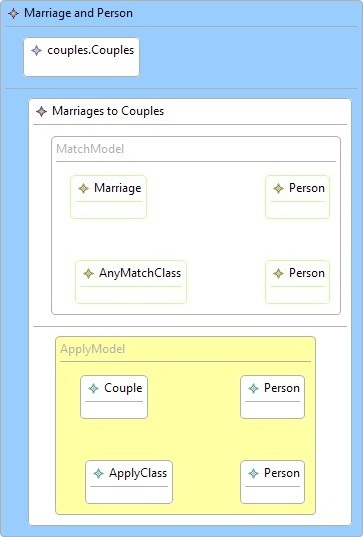
\includegraphics[scale=0.7]{imgs/second_rule_skeleton_2.jpg}
  \caption{Second Rule with class names.}
  \label{fig:second_rule_skeleton_2}
\end{center}
\end{figure}

The generated elements \emph{Couple} and \emph{Person's} need to be associated
with each other and with the root element \emph{CouplesSet} according to the
\emph{Couples} metamodel. To create associations between apply elements you have
to insert \emph{Apply Associations}, click and drag. Insert the needed
associations between the generated elements according to figure
\ref{fig:couple_relations}. Notice that the direction of the
\emph{ApplyAssociations} and their names correspond to the associations
declared in the metamodel. This is very important since \emph{DSLTrans} will
check the generated model correctness and won't allow models that do not conform to
the metamodel.

\begin{figure}[h]
\begin{center}
  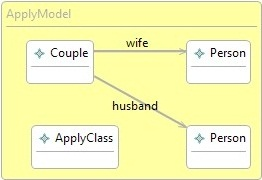
\includegraphics[scale=0.7]{imgs/couple_relations.jpg}
  \caption{Generated \emph{Couple} associations.}
  \label{fig:couple_relations}
\end{center}
\end{figure}

The generated \emph{Couples} need to be related to the root element
\emph{CouplesSet}. Set the properties of the last \emph{ApplyClass} and insert
the association as shown in figure \ref{fig:couple_relations_2}.

\begin{figure}[h]
\begin{center}
  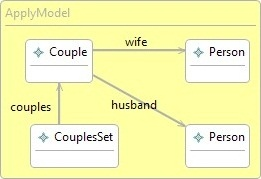
\includegraphics[scale=0.7]{imgs/couple_relations_2.jpg}
  \caption{Generated \emph{Couple} associations with \emph{CouplesSet}.}
  \label{fig:couple_relations_2}
\end{center}
\end{figure}

If you start asking why do we want to generate more \emph{CouplesSet} elements,
then you are in the right track! In this rule you want to add new elements
(\emph{Couple} and \emph{Persons}) but connect them to the previously
generated \emph{CouplesSet} element. How do you say in \emph{DSLTrans} that you
don't want to generate a new \emph{CouplesSet} element but instead want to
use the previously generated one? The answer is to add a
\emph{PositiveBackwardRestriction} between the generated element and one of the
elements that generated it. In this case the generator element is the
\emph{GenealogyTree} and the generated one is the \emph{CouplesSet}. Insert a
\emph{PositiveBackwardRestriction} between the \emph{GenealogyTree} and the
\emph{CouplesSet} and set the required properties so that the \emph{Rule} looks
like the one in figure \ref{fig:rule_without_match_pattern}. Don't forget to set
the appropriate \emph{Package Names}, it's one of the most common errors (see
section \ref{sec:faq}).

\begin{figure}[h]
\begin{center}
  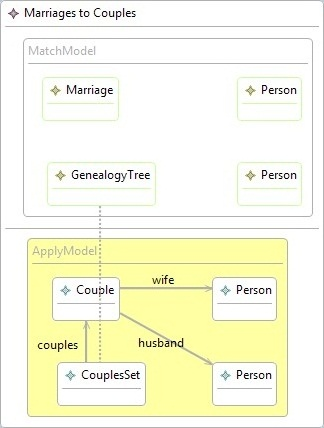
\includegraphics[scale=0.7]{imgs/rule_without_match_pattern.jpg}
  \caption{Rule with a \emph{PositiveBackwardRestriction}.}
  \label{fig:rule_without_match_pattern}
\end{center}
\end{figure}

The apply pattern of the \emph{Rule} is complete and the match elements only
need associations between them. To express that the two
\emph{Person's} are in the same \emph{Marriage}, you have
\emph{PositiveMatchAssociations}. They work much in the same way as the
\emph{ApplyAssociations} in the apply pattern, except they are inserted among
match elements. Insert the required associations so that your match pattern
looks like the one in figure \ref{fig:match_pattern_marriages}.

\begin{figure}[h]
\begin{center}
  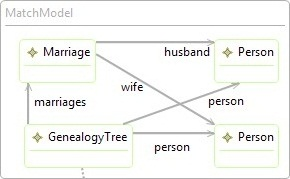
\includegraphics[scale=0.7]{imgs/match_pattern_marriages.jpg}
  \caption{Match pattern with \emph{PositiveMatchAssociations}.}
  \label{fig:match_pattern_marriages}
\end{center}
\end{figure}

Now the rule (and the transformation) is almost complete. However, an important
detail is missing and without it the transformation won't work: when using
\emph{PositiveBackwardRestrictions} you are matching previously generated and
generator elements. \emph{DSLTranslator} internally keeps track of these elements but
only if you say so, or else executing a large transformation would consume a
lot of memory. In order to tell \emph{DSLTranslator} to save traceability links between
generated and generator elements you have to place an \emph{ApplyAttribute}
in the generated elements in the moment they are first created and then use the
same \emph{ApplyAttribute} to refer to them in later \emph{Layers}. It's like
using variables inside a transformation. Go back to the first layer in the
transformation and assign an \emph{ApplyAttribute} to the \emph{CouplesSet}
element and place an \emph{Atom} inside it with the value \emph{Root Element}
(see figure \ref{fig:root_elements_match_attr}). Note that you have to leave the
\emph{Attribute Name} property of the \emph{ApplyAttribute} empty.

\begin{figure}[h]
\begin{center}
  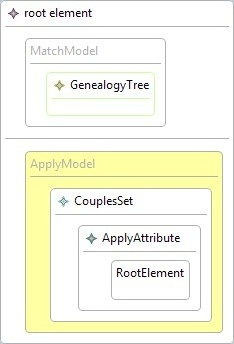
\includegraphics[scale=0.7]{imgs/root_elements_match_attr.jpg}
  \caption{Root elements rule with \emph{ApplyAttribute}.}
  \label{fig:root_elements_match_attr}
\end{center}
\end{figure}

Now in the second \emph{Layer}, add an \emph{ApplyAttribute} with the same
\emph{Atom} value in the \emph{CouplesSet} element, as in figure
\ref{fig:second_layer_rule_with_apply_attr}.

\begin{figure}[h]
\begin{center}
  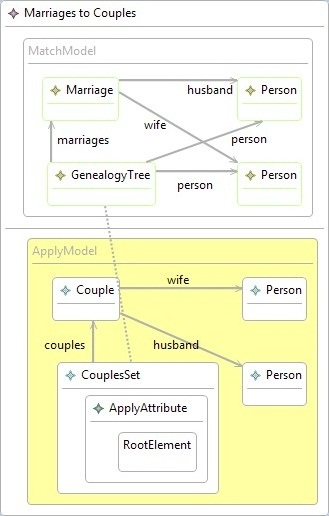
\includegraphics[scale=0.7]{imgs/second_layer_rule_with_apply_attr.jpg}
  \caption{\emph{CouplesSet} element with \emph{ApplyAttribute}.}
  \label{fig:second_layer_rule_with_apply_attr}
\end{center}
\end{figure}

Executing the transformation now should produce a result similar to the one in
figure \ref{fig:result_without_attributes}.

\begin{figure}[h]
\begin{center}
  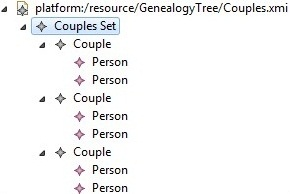
\includegraphics[scale=0.7]{imgs/result_without_attributes.jpg}
  \caption{\emph{Couples} result model with missing attributes.}
  \label{fig:result_without_attributes}
\end{center}
\end{figure}

All the generated elements' attributes are missing. Apart from the
\emph{ApplyAttribute} (with no name) that you set for the root element, you
didn't create any attribute for other elements.

You need to copy the name attribute from each element in the input model to
the output model. To do that, insert an \emph{ApplyAttribute}, name it according to
figure \ref{fig:rule_with_attrs_ref} , insert \emph{AttributeRef} (Objects)
inside each \emph{ApplyAttribute}, place \emph{MatchAttributes} inside the relevant elements
in the match pattern and insert \emph{AttributeRefs} (Connections) between the
\emph{ApplyAttributes} and the corresponding \emph{MatchAttributes}. The
resulting \emph{Rule} is in figure \ref{fig:rule_with_attrs_ref}.

\begin{figure}[h]
\begin{center}
  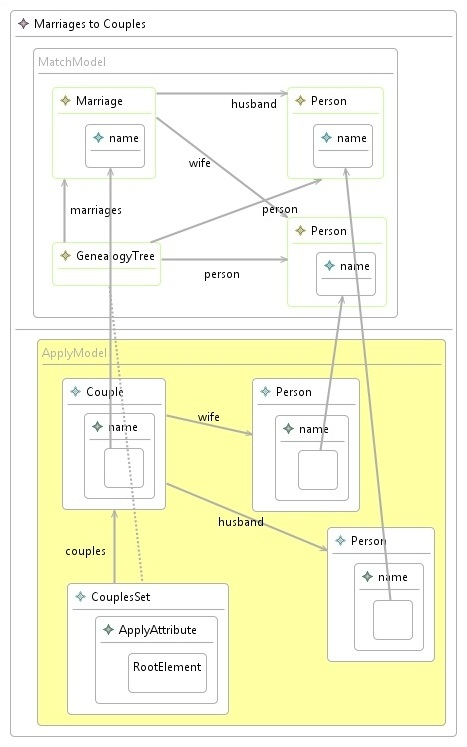
\includegraphics[scale=0.7]{imgs/rule_with_attrs_ref.jpeg}
  \caption{Rule with \emph{MatchAttributes} and \emph{AttributeRefs}.}
  \label{fig:rule_with_attrs_ref}
\end{center}
\end{figure}

You just told \emph{DSLTranslator} to copy the \emph{name} attributes from the
elements matched in the input model and paste them in the applied elements.

Finally, you can run the transformation against any model (expressed in
\emph{GenealogyTree.xmi}) and get the set of couples (in the \emph{Couples.xmi}
resulting file). The result for our case study is shown in figure
\ref{fig:first_transformatio_result}.

\begin{figure}[h]
\begin{center}
  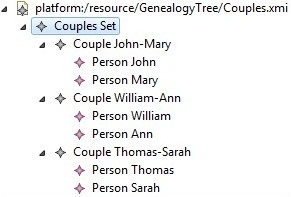
\includegraphics[scale=0.7]{imgs/first_transformatio_result.jpg}
  \caption{Final result.}
  \label{fig:first_transformatio_result}
\end{center}
\end{figure}

With this transformation you are able to obtain a model of the existing couples
in a genealogical tree. But wouldn't it be great if you were able to see the
relations between couples. Who is the oldest couple? And the youngest? In the
next session you will learn to build a transformation for that.

\clearpage

\subsection{Transformation Partitioning}

In the previous section you learned how to build a simple transformation to
generate a flat list of couples model out of a genealogical tree model. Now you
will learn to do more than that: you will generate a hierarchical set of couples
based on their age, i.e., the oldest couple will the the parent of all the other
couples, and so on.

In order to build this transformation you will follow a slightly different
approach: you will first transform each individual element, then you will look
at groups of elements and create relations in the output model, thus
connecting all the ``loose'' elements. Figure \ref{fig:transformation_natural}
gives an example of the processing stages of a transformation following this
approach: first individual elements are considered, then it looks to bigger and
bigger sets of elements; at the end, all the elements that where generated but
are not ``attached'' to something are discarded.

\begin{figure}[h]
\begin{center}
  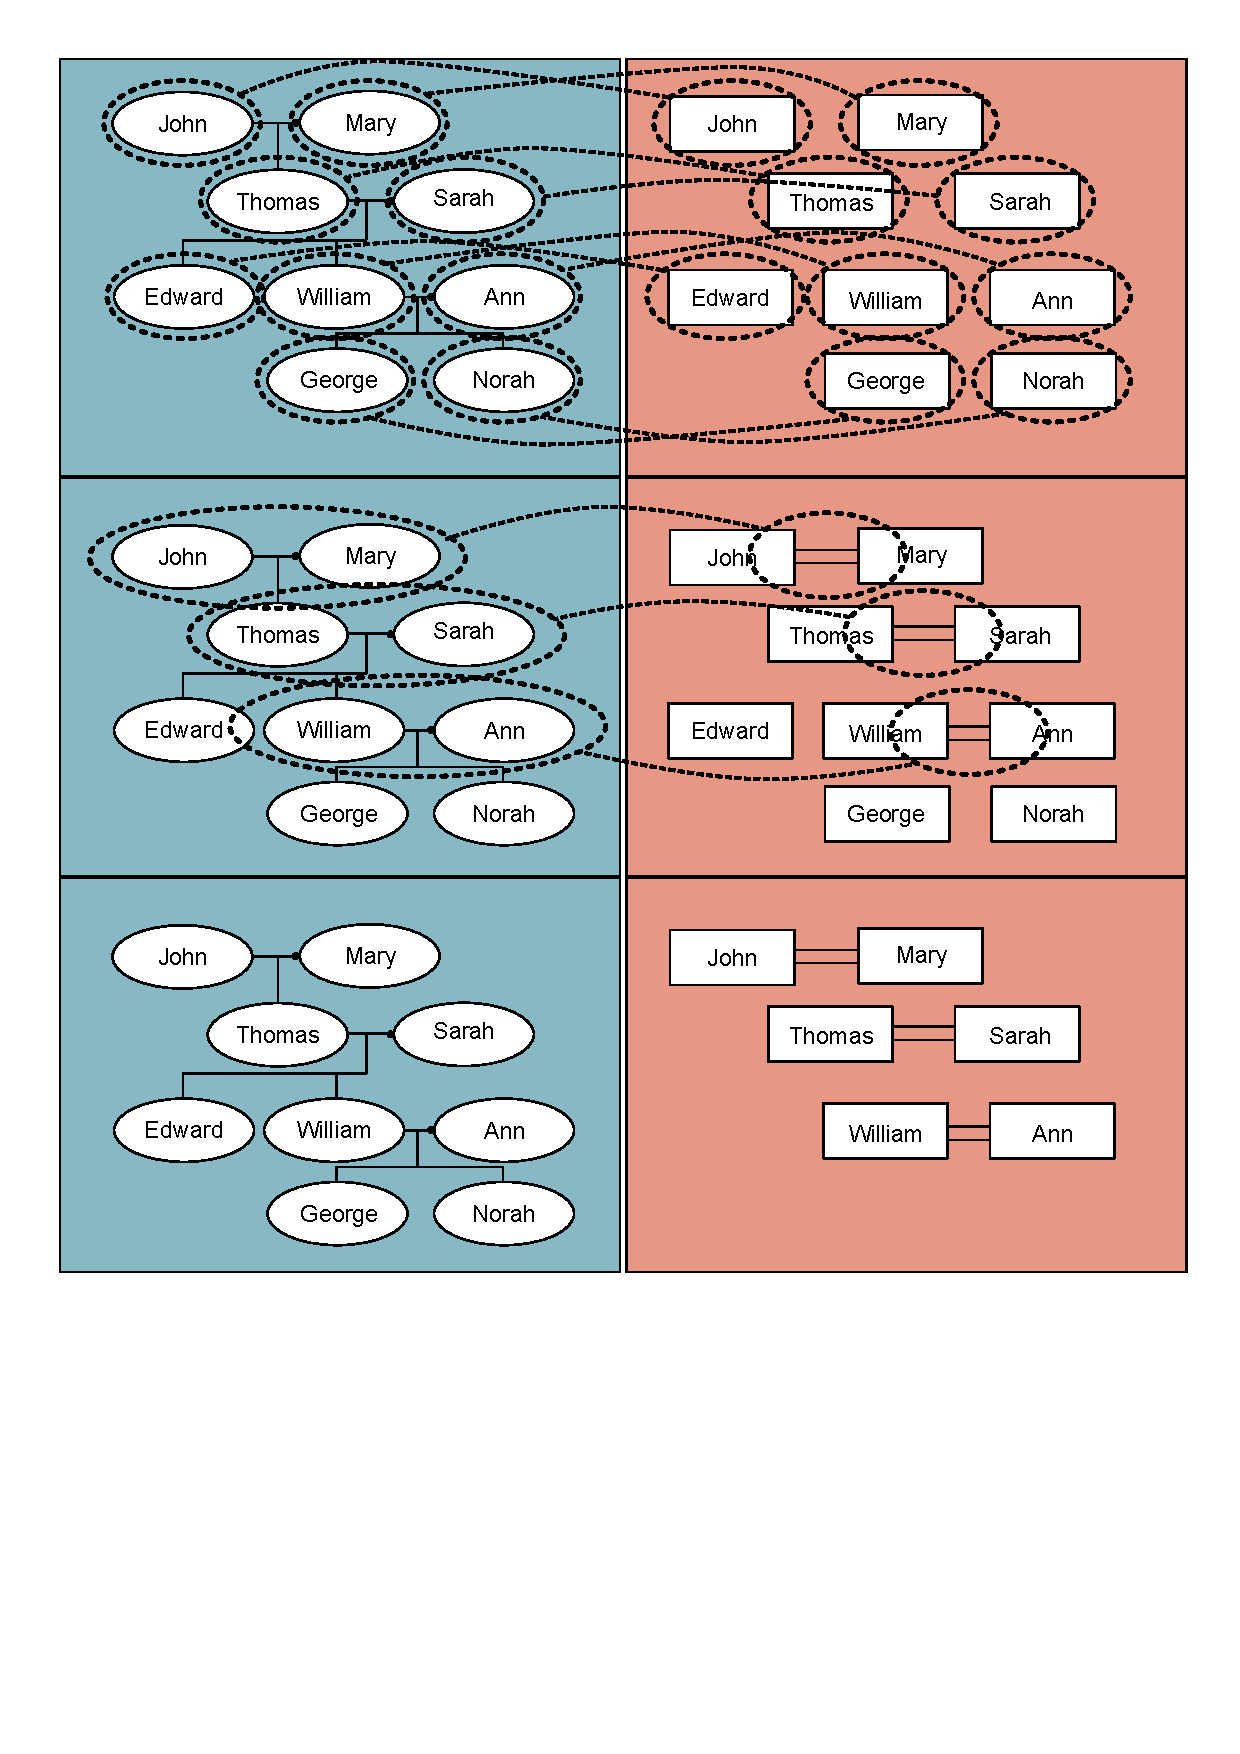
\includegraphics[scale=0.6, trim=0.9cm 8cm 0.7cm 0.8cm,
  clip]{imgs/transformation_natural.pdf}
  \caption{Transformation partitioning approach.}
  \label{fig:transformation_natural}
\end{center}
\end{figure}

Since you already have the required metamodels and an example model from
previous section, all we have to do is to create a new \emph{DSLTrans} transformation,
add a \emph{FilePort}, a \emph{Rule}, the \emph{MetaModelIdentifiers} needed to
get a transformation like the one shown in figure \ref{fig:part_trans_rule_bas}.

\begin{figure}[h]
\begin{center}
  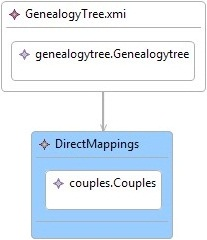
\includegraphics[scale=0.7]{imgs/part_trans_rule_bas.jpg}
  \caption{Basic transformation skeleton.}
  \label{fig:part_trans_rule_bas}
\end{center}
\end{figure}

Has described earlier, in this approach you first identify what each element in
the input model \emph{means} in the output model.

\begin{itemize}
  \item Each \emph{Person} in the \emph{GenealogyTree} is a \emph{Person} in
  \emph{Couples};
  \item Each \emph{Marriage} can be seen as a \emph{Couple};
  \item The \emph{GenealogyTree} element is the \emph{CouplesSet} element.
\end{itemize}

With these three mappings you should create three simple rules in the first
layer (see figure \ref{fig:first_rule_direct_mappings}). Don't forget to set the
\emph{Package Name} properties for each \emph{AnyMatchClass} and
\emph{ApplyClasses}.


\begin{figure}[h]
\begin{center}
  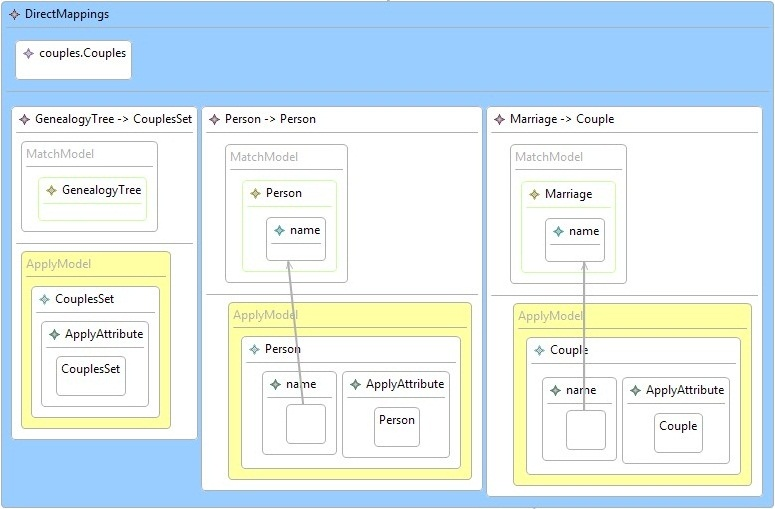
\includegraphics[scale=0.7]{imgs/first_rule_direct_mappings.jpg}
  \caption{First layer direct mappings.}
  \label{fig:first_rule_direct_mappings}
\end{center}
\end{figure}

Figure \ref{fig:first_layer_result} shows the result of executing the layer
you've just built. Notice that, internally, \emph{DSLTranslator} keeps trace of
the generated elements and generator elements. We call that \emph{traceability
links} (in the figure they are represented as dashed lines between generated
and generator elements). This feature makes it possible to later match those
elements and complete the transformation.

\begin{figure}[h]
\begin{center}
  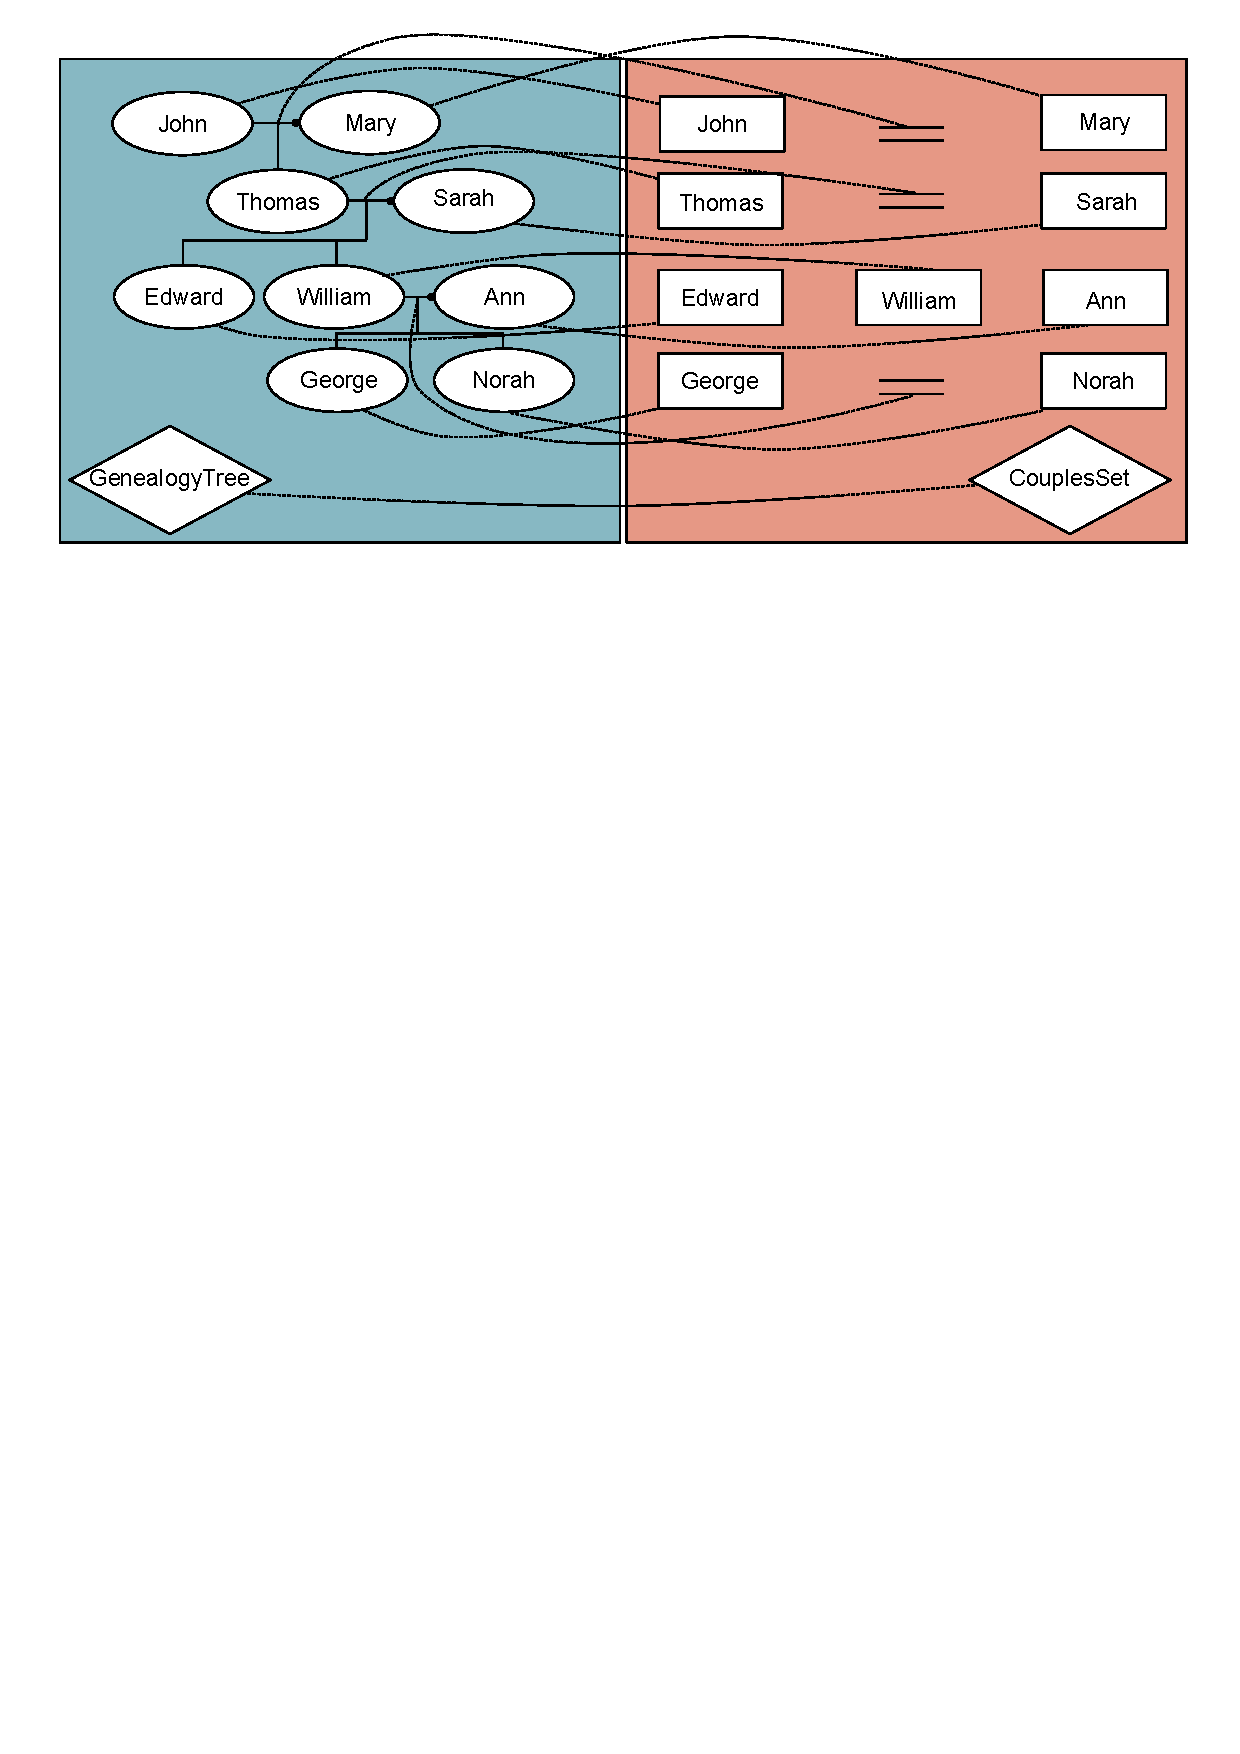
\includegraphics[scale=0.6, trim=0.8cm 20.3cm 0.7cm 0.3cm,
  clip]{imgs/first_layer_result.pdf}
  \caption{Resulting models after executing the mappings layer.}
  \label{fig:first_layer_result}
\end{center}
\end{figure}

Now it is necessary to match the possible relations between elements in the
input model and translate that to association (and sometimes new elements) in
the output model. What does the relation of \emph{husband} between a \emph{Marriage}
and a \emph{Person} in the \emph{GenealogyTree} mean? Insert a new \emph{Layer}
and all the elements needed to get it like the one shown in figure
\ref{fig:second_layers_relations}.

\begin{figure}[h]
\begin{center}
  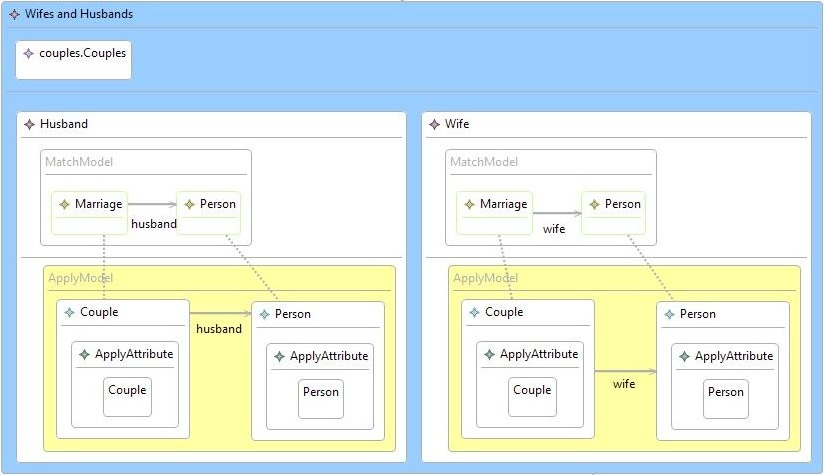
\includegraphics[width=\textwidth]{imgs/second_layers_relations.jpg}
  \caption{Husband and Wife relations layer.}
  \label{fig:second_layers_relations}
\end{center}
\end{figure}

The first layer generates a set of loose elements in the output model, the
second one connects people with couples as figure \ref{fig:second_layer_result}
illustrates. The only thing missing is to connect the couples in a hierarchical
fashion so go ahead and build a third \emph{Layer} connected to the second one
and with the proper \emph{MetaModelIdentifier} but without any rule.

\begin{figure}[h]
\begin{center}
  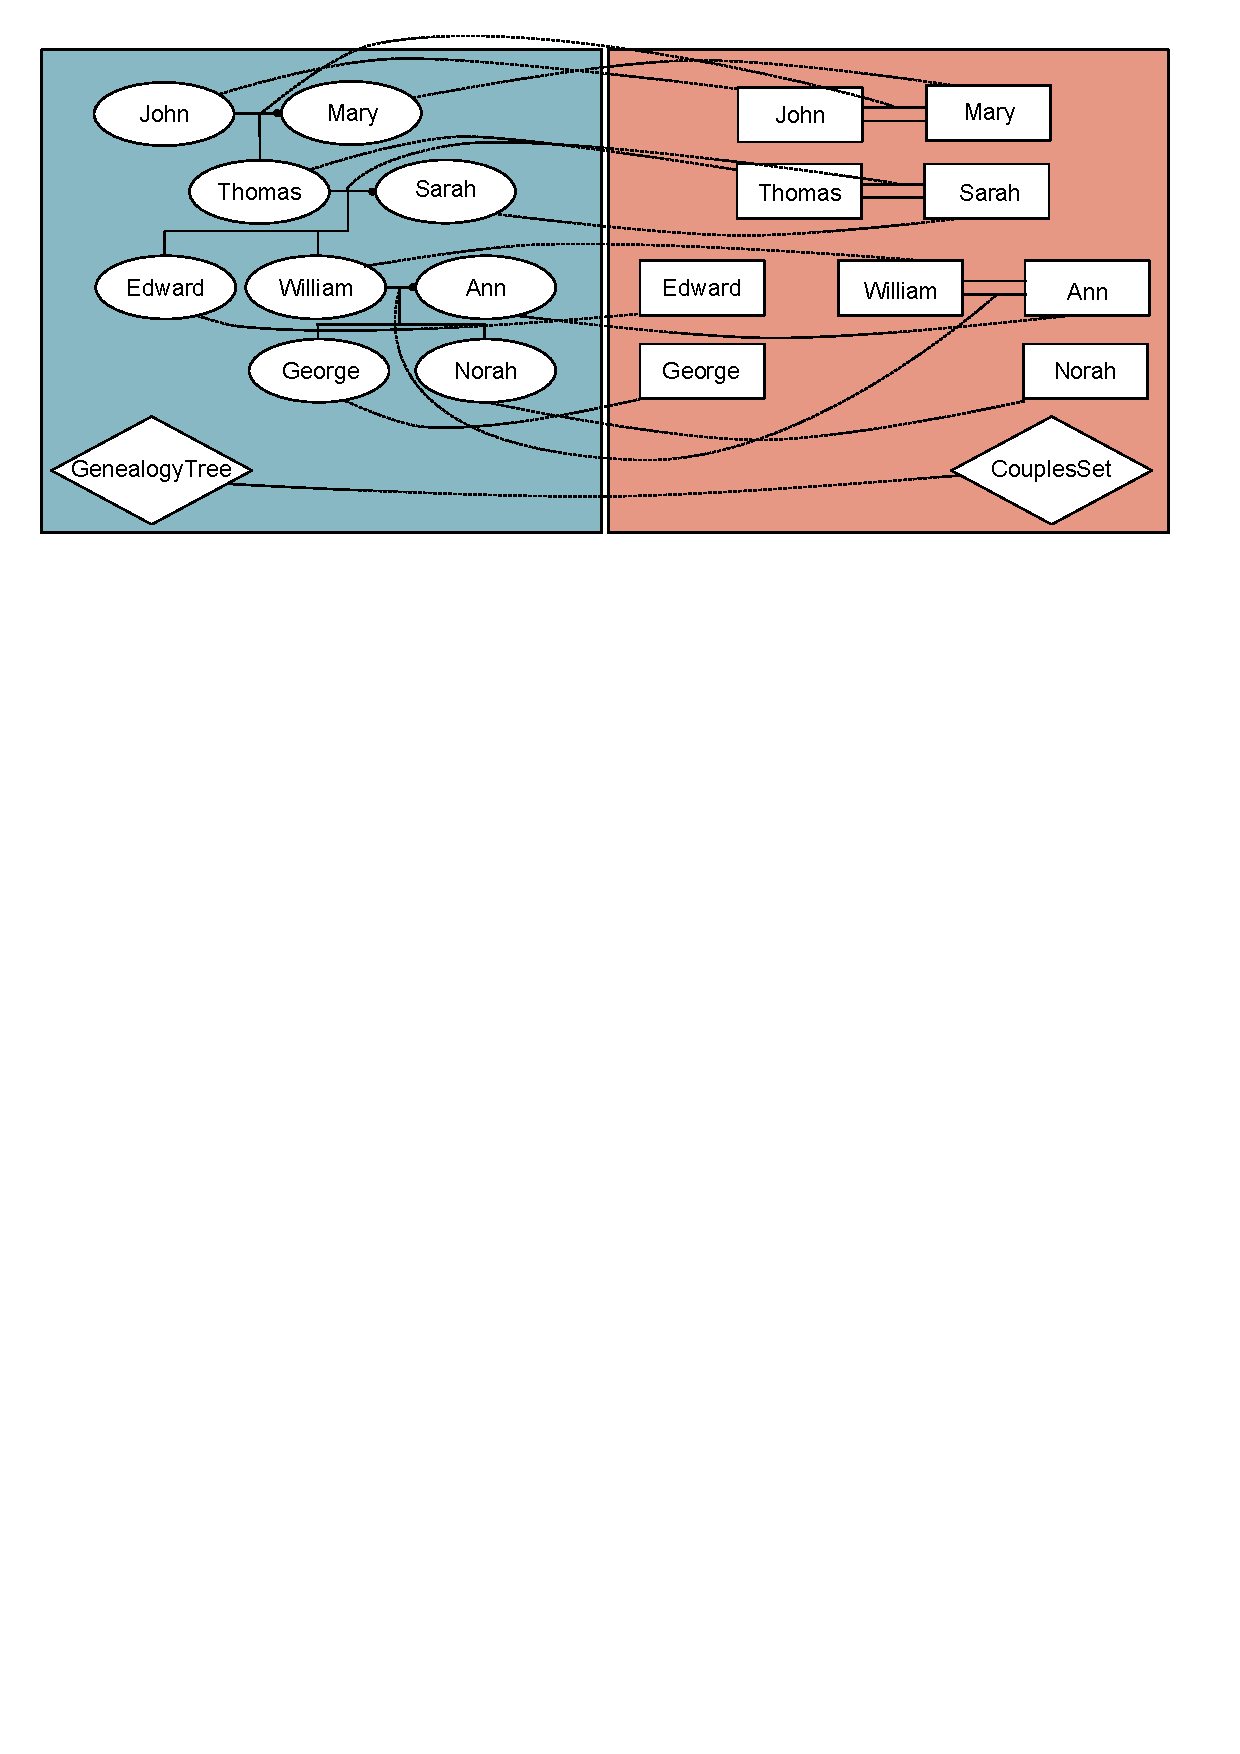
\includegraphics[scale=0.6, trim=0.5cm 20.4cm 1.0cm 0.6cm,
  clip]{imgs/second_layer_result.pdf}
  \caption{Resulting models after executing the second layer.}
  \label{fig:second_layer_result}
\end{center}
\end{figure}

How do you know that a couple is a \emph{child} or a \emph{parent}?
If \emph{John} is married to \emph{Mary} and one (or more) of their children is
married to someone else then \emph{John's} \emph{Marriage} is a parent of its
children's \emph{Marriages}.

The two rules shown in figure \ref{fig:couples_hierarchy_rules} express this
concept. Notice that the two cases have to be considered since there are two
ways of being in a marriage (husband or wife) in the \emph{GenealogyTree} model.

\begin{figure}[h]
\begin{center}
  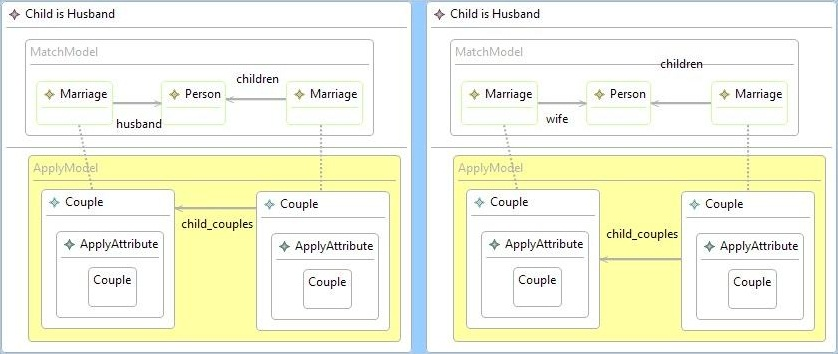
\includegraphics[width=\textwidth]{imgs/couples_hierarchy_rules.jpg}
  \caption{Couples hierarchy rules.}
  \label{fig:couples_hierarchy_rules}
\end{center}
\end{figure}

After executing the transformation (with the rules shown in figure
\ref{fig:couples_hierarchy_rules} added) you will have as a result something
like figure \ref{fig:third_layer_result_inc}.

\begin{figure}[h]
\begin{center}
  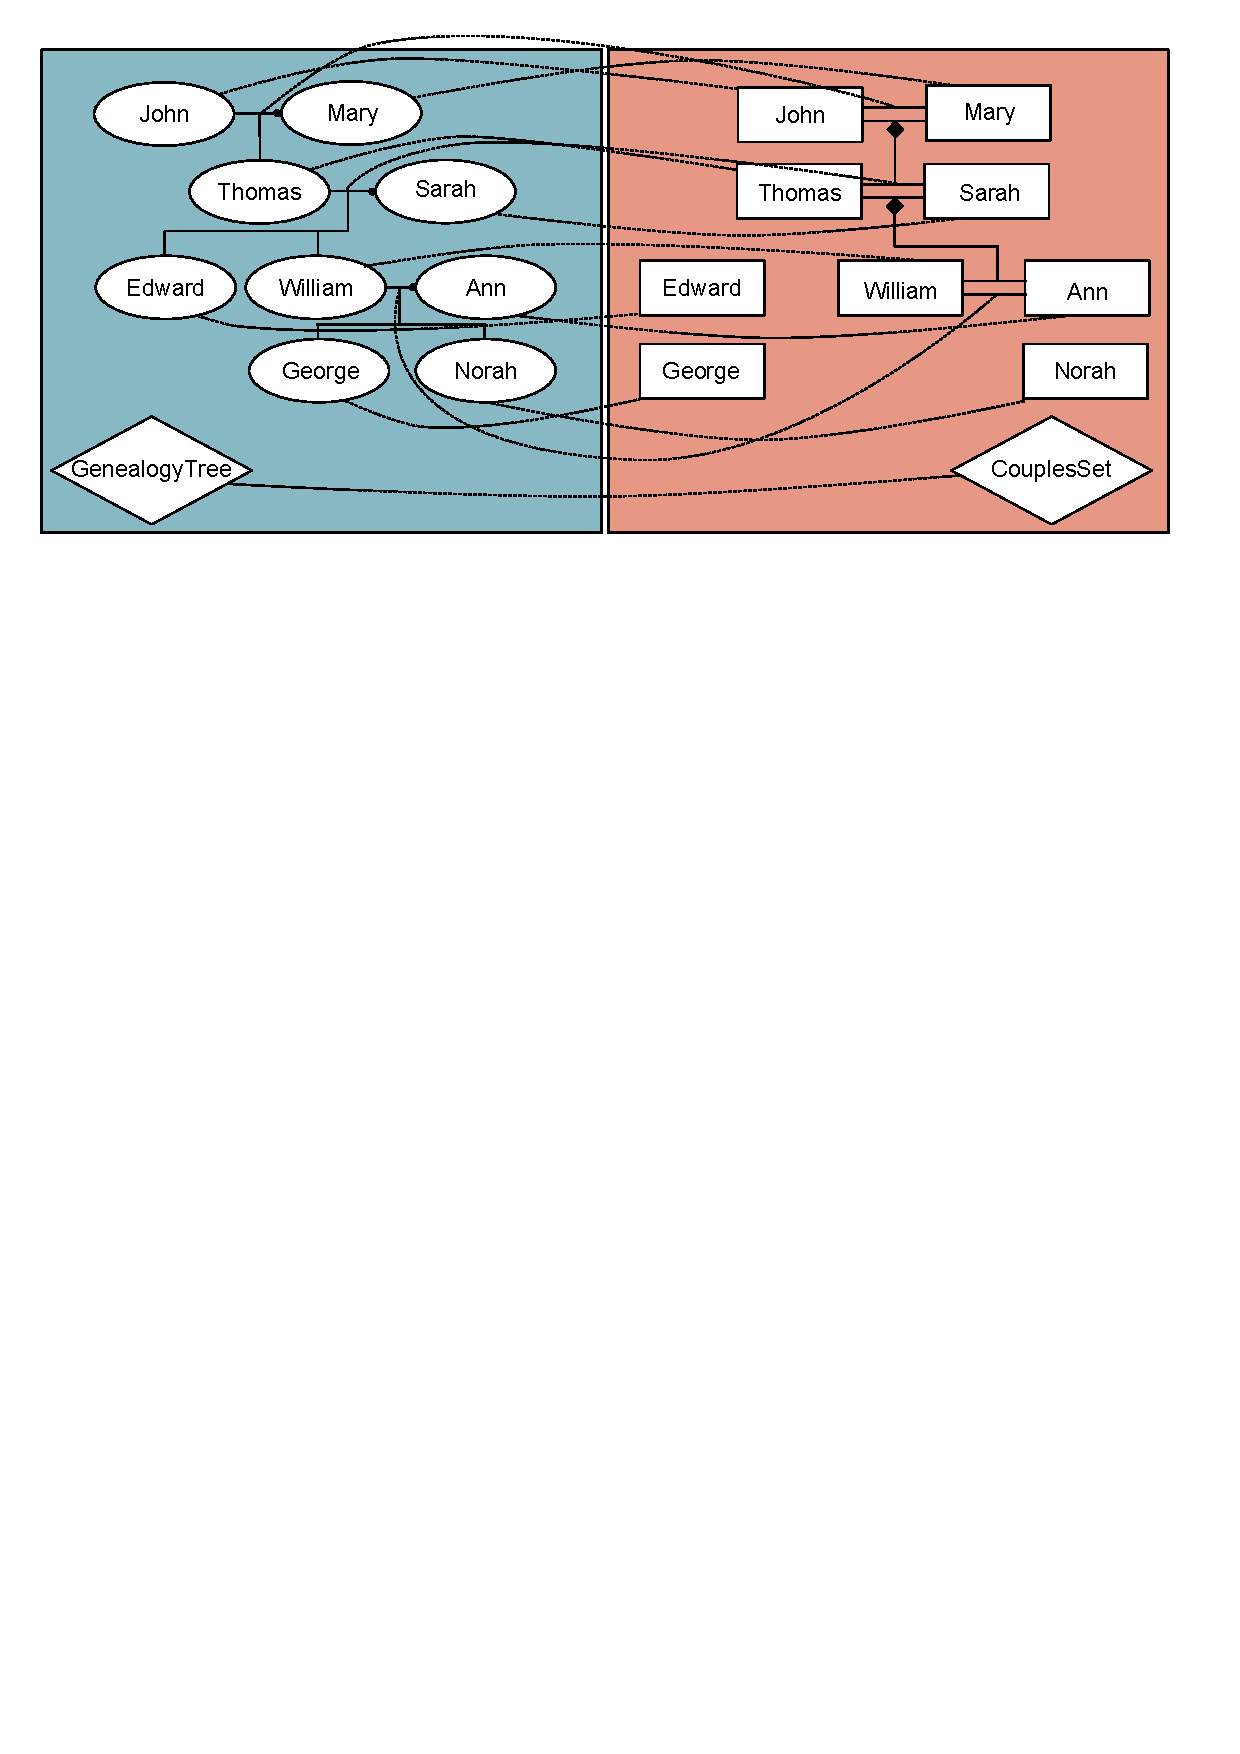
\includegraphics[scale=0.6, trim=0.5cm 20.4cm 1.0cm 0.6cm,
  clip]{imgs/third_layer_result_inc.pdf}
  \caption{Resulting models after executing the third layer's two rules.}
  \label{fig:third_layer_result_inc}
\end{center}
\end{figure} 

What about the oldest couple? According to the rules defined previously the
oldest couple (in this case \emph{John} and \emph{Mary}) is not contained
anywhere in the model. If you don't make a rule for this couple none of the
other younger couples will be visible in the output model. Figure
\ref{fig:root_couple_rule} shows the rule you need to add to the third layer in
order to match the oldest couple and connect it to the \emph{CouplesSet}
element.

\begin{figure}[h]
\begin{center}
  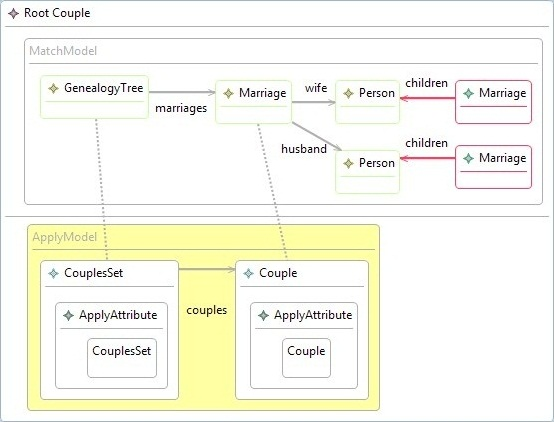
\includegraphics[scale=0.7]{imgs/root_couple_rule.jpg}
  \caption{Root couple rule.}
  \label{fig:root_couple_rule}
\end{center}
\end{figure}

The rule in figure \ref{fig:root_couple_rule} matches a couple whose individuals
(\emph{husband} and \emph{wife}) aren't children of anyone else. Notice the way
to express a nonexistent class (and association) in \emph{DSLTrans}.

After the execution of this last rule all the relevant elements are connected to
the output model and hence, are displayed in the final result. The elements that
are generated during the transformation (for instance, \emph{George},
\emph{Edward} and \emph{Norah}) and are not (in)directly contained in the output
model root element (in this case, the \emph{CouplesSet} element) do not appear
in the final result as shown in figures \ref{fig:third_layer_result} and
\ref{fig:third_layer_results}.

\begin{figure}[h]
\begin{center}
  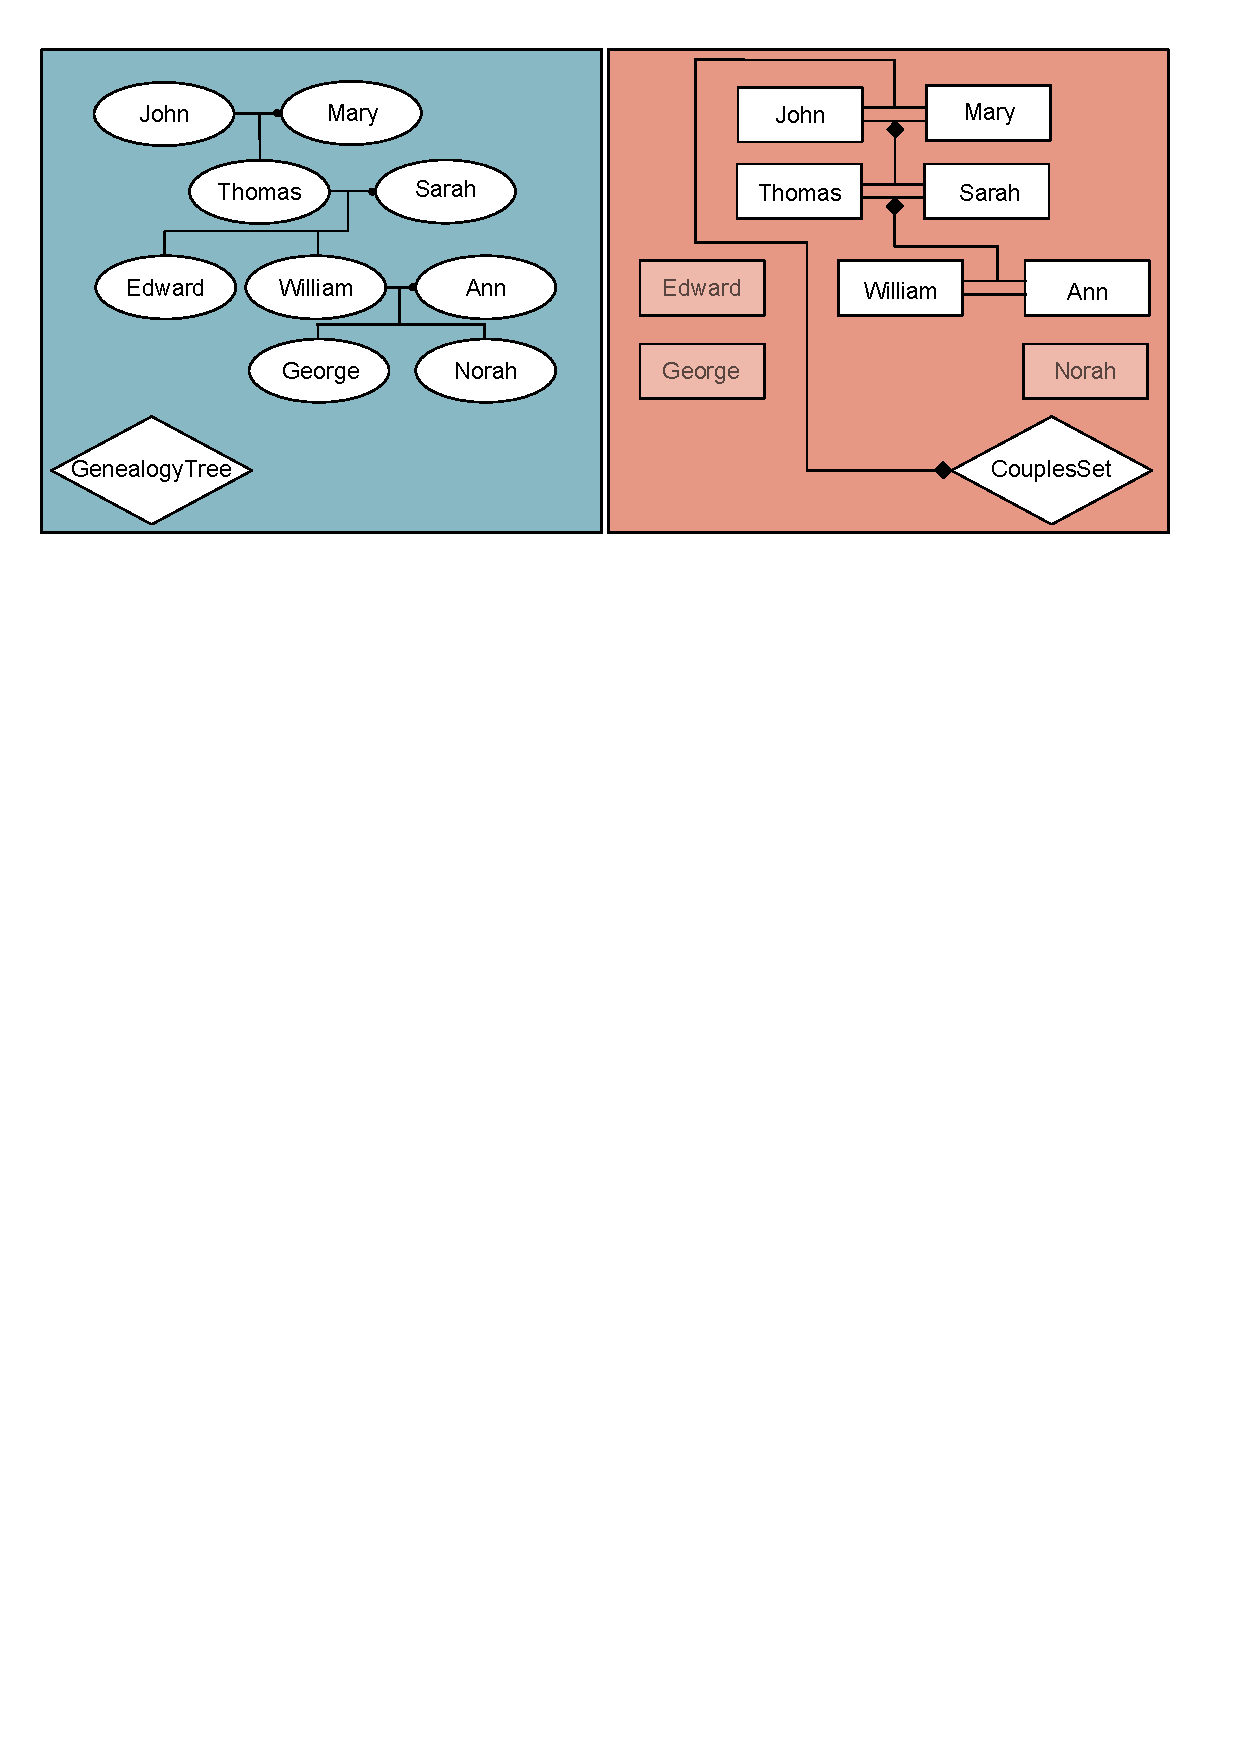
\includegraphics[scale=0.6, trim=0.5cm 20.4cm 1.0cm 0.6cm,
  clip]{imgs/third_layer_result.pdf}
  \caption{Resulting models after executing the transformation.}
  \label{fig:third_layer_result}
\end{center}
\end{figure}

\begin{figure}[h]
\begin{center}
  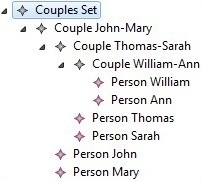
\includegraphics[scale=0.7]{imgs/third_layer_results.jpg}
  \caption{Resulting \emph{XMI} file.}
  \label{fig:third_layer_results}
\end{center}
\end{figure}

In the next sections you will be able to learn more about each element of the
\emph{DSLTrans} language individually. It is up to you to combine
the elements in order to create almost any rule you need in a readable and
elegant manner.

\clearpage